\documentclass{beamer}

% xcolor and define colors -------------------------
\usepackage{xcolor}

% https://www.viget.com/articles/color-contrast/
\definecolor{purple}{HTML}{5601A4}
\definecolor{navy}{HTML}{0D3D56}
\definecolor{ruby}{HTML}{9a2515}
\definecolor{alice}{HTML}{107895}
\definecolor{daisy}{HTML}{EBC944}
\definecolor{coral}{HTML}{F26D21}
\definecolor{kelly}{HTML}{829356}
\definecolor{cranberry}{HTML}{E64173}
\definecolor{jet}{HTML}{131516}
\definecolor{asher}{HTML}{555F61}
\definecolor{slate}{HTML}{314F4F}

% Mixtape Sessions
\definecolor{picton-blue}{HTML}{00b7ff}
\definecolor{violet-red}{HTML}{ff3881}
\definecolor{sun}{HTML}{ffaf18}
\definecolor{electric-violet}{HTML}{871EFF}

% Main theme colors
\definecolor{accent}{HTML}{00b7ff}
\definecolor{accent2}{HTML}{871EFF}
\definecolor{gray100}{HTML}{f3f4f6}
\definecolor{gray800}{HTML}{1F292D}


% Beamer Options -------------------------------------

% Background
\setbeamercolor{background canvas}{bg = white}

% Change text margins
\setbeamersize{text margin left = 15pt, text margin right = 15pt} 

% \alert
\setbeamercolor{alerted text}{fg = accent2}

% Frame title
\setbeamercolor{frametitle}{bg = white, fg = jet}
\setbeamercolor{framesubtitle}{bg = white, fg = accent}
\setbeamerfont{framesubtitle}{size = \small, shape = \itshape}

% Block
\setbeamercolor{block title}{fg = white, bg = accent2}
\setbeamercolor{block body}{fg = gray800, bg = gray100}

% Title page
\setbeamercolor{title}{fg = gray800}
\setbeamercolor{subtitle}{fg = accent}

%% Custom \maketitle and \titlepage
\setbeamertemplate{title page}
{
    %\begin{centering}
        \vspace{20mm}
        {\Large \usebeamerfont{title}\usebeamercolor[fg]{title}\inserttitle}\\
        {\large \itshape \usebeamerfont{subtitle}\usebeamercolor[fg]{subtitle}\insertsubtitle}\\ \vspace{10mm}
        {\insertauthor}\\
        {\color{asher}\small{\insertdate}}\\
    %\end{centering}
}

% Table of Contents
\setbeamercolor{section in toc}{fg = accent!70!jet}
\setbeamercolor{subsection in toc}{fg = jet}

% Button 
\setbeamercolor{button}{bg = accent}

% Remove navigation symbols
\setbeamertemplate{navigation symbols}{}

% Table and Figure captions
\setbeamercolor{caption}{fg=jet!70!white}
\setbeamercolor{caption name}{fg=jet}
\setbeamerfont{caption name}{shape = \itshape}

% Bullet points

%% Fix left-margins
\settowidth{\leftmargini}{\usebeamertemplate{itemize item}}
\addtolength{\leftmargini}{\labelsep}

%% enumerate item color
\setbeamercolor{enumerate item}{fg = accent}
\setbeamerfont{enumerate item}{size = \small}
\setbeamertemplate{enumerate item}{\insertenumlabel.}

%% itemize
\setbeamercolor{itemize item}{fg = accent!70!white}
\setbeamerfont{itemize item}{size = \small}
\setbeamertemplate{itemize item}[circle]

%% right arrow for subitems
\setbeamercolor{itemize subitem}{fg = accent!60!white}
\setbeamerfont{itemize subitem}{size = \small}
\setbeamertemplate{itemize subitem}{$\rightarrow$}

\setbeamertemplate{itemize subsubitem}[square]
\setbeamercolor{itemize subsubitem}{fg = jet}
\setbeamerfont{itemize subsubitem}{size = \small}







% Links ----------------------------------------------

\usepackage{hyperref}
\hypersetup{
  colorlinks = true,
  linkcolor = accent2,
  filecolor = accent2,
  urlcolor = accent2,
  citecolor = accent2,
}


% Line spacing --------------------------------------
\usepackage{setspace}
\setstretch{1.1}


% \begin{columns} -----------------------------------
\usepackage{multicol}


% Fonts ---------------------------------------------
% Beamer Option to use custom fonts
\usefonttheme{professionalfonts}

% \usepackage[utopia, smallerops, varg]{newtxmath}
% \usepackage{utopia}
\usepackage[sfdefault,light]{roboto}

% Small adjustments to text kerning
\usepackage{microtype}



% Remove annoying over-full box warnings -----------
\vfuzz2pt 
\hfuzz2pt


% Table of Contents with Sections
\setbeamerfont{myTOC}{series=\bfseries, size=\Large}
\AtBeginSection[]{
        \frame{
            \frametitle{Roadmap}
            \tableofcontents[current]   
        }
    }


% Tables -------------------------------------------
% Tables too big
% \begin{adjustbox}{width = 1.2\textwidth, center}
\usepackage{adjustbox}
\usepackage{array}
\usepackage{threeparttable, booktabs, adjustbox}
    
% Fix \input with tables
% \input fails when \\ is at end of external .tex file
\makeatletter
\let\input\@@input
\makeatother

% Tables too narrow
% \begin{tabularx}{\linewidth}{cols}
% col-types: X - center, L - left, R -right
% Relative scale: >{\hsize=.8\hsize}X/L/R
\usepackage{tabularx}
\newcolumntype{L}{>{\raggedright\arraybackslash}X}
\newcolumntype{R}{>{\raggedleft\arraybackslash}X}
\newcolumntype{C}{>{\centering\arraybackslash}X}

% Figures

% \imageframe{img_name} -----------------------------
% from https://github.com/mattjetwell/cousteau
\newcommand{\imageframe}[1]{%
    \begin{frame}[plain]
        \begin{tikzpicture}[remember picture, overlay]
            \node[at = (current page.center), xshift = 0cm] (cover) {%
                \includegraphics[keepaspectratio, width=\paperwidth, height=\paperheight]{#1}
            };
        \end{tikzpicture}
    \end{frame}%
}

% subfigures
\usepackage{subfigure}


% Highlight slide -----------------------------------
% \begin{transitionframe} Text \end{transitionframe}
% from paulgp's beamer tips
\newenvironment{transitionframe}{
    \setbeamercolor{background canvas}{bg=accent!40!black}
    \begin{frame}\color{accent!10!white}\LARGE\centering
}{
    \end{frame}
}


% Table Highlighting --------------------------------
% Create top-left and bottom-right markets in tabular cells with a unique matching id and these commands will outline those cells
\usepackage[beamer,customcolors]{hf-tikz}
\usetikzlibrary{calc}
\usetikzlibrary{fit,shapes.misc}

% To set the hypothesis highlighting boxes red.
\newcommand\marktopleft[1]{%
    \tikz[overlay,remember picture] 
        \node (marker-#1-a) at (0,1.5ex) {};%
}
\newcommand\markbottomright[1]{%
    \tikz[overlay,remember picture] 
        \node (marker-#1-b) at (0,0) {};%
    \tikz[accent!80!jet, ultra thick, overlay, remember picture, inner sep=4pt]
        \node[draw, rectangle, fit=(marker-#1-a.center) (marker-#1-b.center)] {};%
}

\usepackage{breqn} % Breaks lines

\usepackage{amsmath}
\usepackage{mathtools}

\usepackage{pdfpages} % \includepdf

\usepackage{listings} % R code
\usepackage{verbatim} % verbatim

% Video stuff
\usepackage{media9}

% packages for bibs and cites
\usepackage{natbib}
\usepackage{har2nat}
\newcommand{\possessivecite}[1]{\citeauthor{#1}'s \citeyearpar{#1}}
\usepackage{breakcites}
\usepackage{alltt}

% Setup math operators
\DeclareMathOperator{\E}{E} \DeclareMathOperator{\tr}{tr} \DeclareMathOperator{\se}{se} \DeclareMathOperator{\I}{I} \DeclareMathOperator{\sign}{sign} \DeclareMathOperator{\supp}{supp} \DeclareMathOperator{\plim}{plim}
\DeclareMathOperator*{\dlim}{\mathnormal{d}\mkern2mu-lim}
\newcommand\independent{\protect\mathpalette{\protect\independenT}{\perp}}
   \def\independenT#1#2{\mathrel{\rlap{$#1#2$}\mkern2mu{#1#2}}}
\newcommand*\colvec[1]{\begin{pmatrix}#1\end{pmatrix}}

\newcommand{\myurlshort}[2]{\href{#1}{\textcolor{gray}{\textsf{#2}}}}


\begin{document}

\imageframe{./lecture_includes/mixtape_did_cover.png}


% ---- Content ----

\section{Differential timing}

\subsection{Bacon decomposition}

\begin{frame}{Differential timing}

\begin{itemize}
\item We covered mostly the simple two group case
\item In the two group case, we can estimate the ATT under parallel trends using OLS with unit and time fixed effects
\item If we have covariates, then we can use TWFE under restrictive assumptions, or we have other options (OR, IPW, DR)
\item Now let's move to a more common scenario where we have more than two groups who get treated at various times
\end{itemize}

\end{frame}

\begin{frame}{2x2 versus differential timing}

\begin{itemize}
	\item For this next part, similar to how we did with Sant'Anna and Zhao (2020), we will decompose TWFE to understand what it needs for unbiasedness under differential timing
	\item All of this is from Goodman-Bacon (2021, forthcoming) though the expression of the weights is from 2018 for personal preference
	\item Goodman-Bacon (2021, forthcoming) shows that parallel trends is \textbf{not enough} for TWFE to be unbiased when treatment adoption is described by differential timing
	\item TWFE with differential timing uses treated groups as controls -- not all estimators do -- and this can introduce bias
\end{itemize}

\end{frame}



\begin{frame}{Decomposition Preview}

\begin{itemize}
\item TWFE estimates a parameter that is a weighted average over all 2x2 in your sample
\item TWFE assigns weights that are a function of sample sizes of each ``group'' and the variance of the treatment dummies for those groups
\end{itemize}

\end{frame}

\begin{frame}{Decomposition (cont.)}

\begin{itemize}
\item TWFE needs two assumptions: that the variance weighted parallel trends are zero (far more parallel trends iow) and no dynamic treatment effects (not the case with 2x2)
\item Under those assumptions, TWFE estimator estimates the variance weighted ATT as a weighted average of all possible ATTs
\end{itemize}

\end{frame}


\begin{frame}{$K^2$ distinct DDs}

Let's look at 3 timing groups (a, b and c) and one untreated group (U).  With 3 timing groups, there are 9 2x2 DDs.  Here they are:


\begin{center}
\begin{tabular}{c|c|c}
\multicolumn{1}{l}{} &
\multicolumn{1}{l}{} &
\multicolumn{1}{l}{} \\
\midrule
a to b & b to a & c to a \\
a to c & b to c & c to b \\
a to U & b to U & c to U \\
\midrule
\end{tabular}
\end{center}

\bigskip

Let's return to a simpler example with only two groups -- a $k$ group treated at $t_k^*$ and an $l$ treated at $t_l^*$ plus an never-treated group called the $U$ untreated group
\end{frame} 


\begin{frame}{Terms and notation}

\begin{itemize}
\item Let there be two treatment groups (k,l) and one untreated group (U)
\item k,l define the groups based on when they receive treatment (differently in time) with k receiving it earlier than l
\item Denote $\overline{D}_k$ as the share of time each group spends in treatment status
\item Denote $\widehat{\delta}_{jb}^{2x2}$ as the canonical $2\times 2$ DD estimator for groups $j$ and b where $j$ is the treatment group and $b$ is the comparison group
\end{itemize}

\end{frame}


\imageframe{./lecture_includes/bacon_goodman_2.png}



\begin{frame}[plain]
$$\widehat{\delta}^{2x2}_{kU} = \bigg ( \overline{y}_k^{post(k)} - \overline{y}_k^{pre(k)} \bigg ) - \bigg ( \overline{y}_U^{post(k)} - \overline{y}_U^{pre(k)} \bigg ) $$
	\begin{figure}
	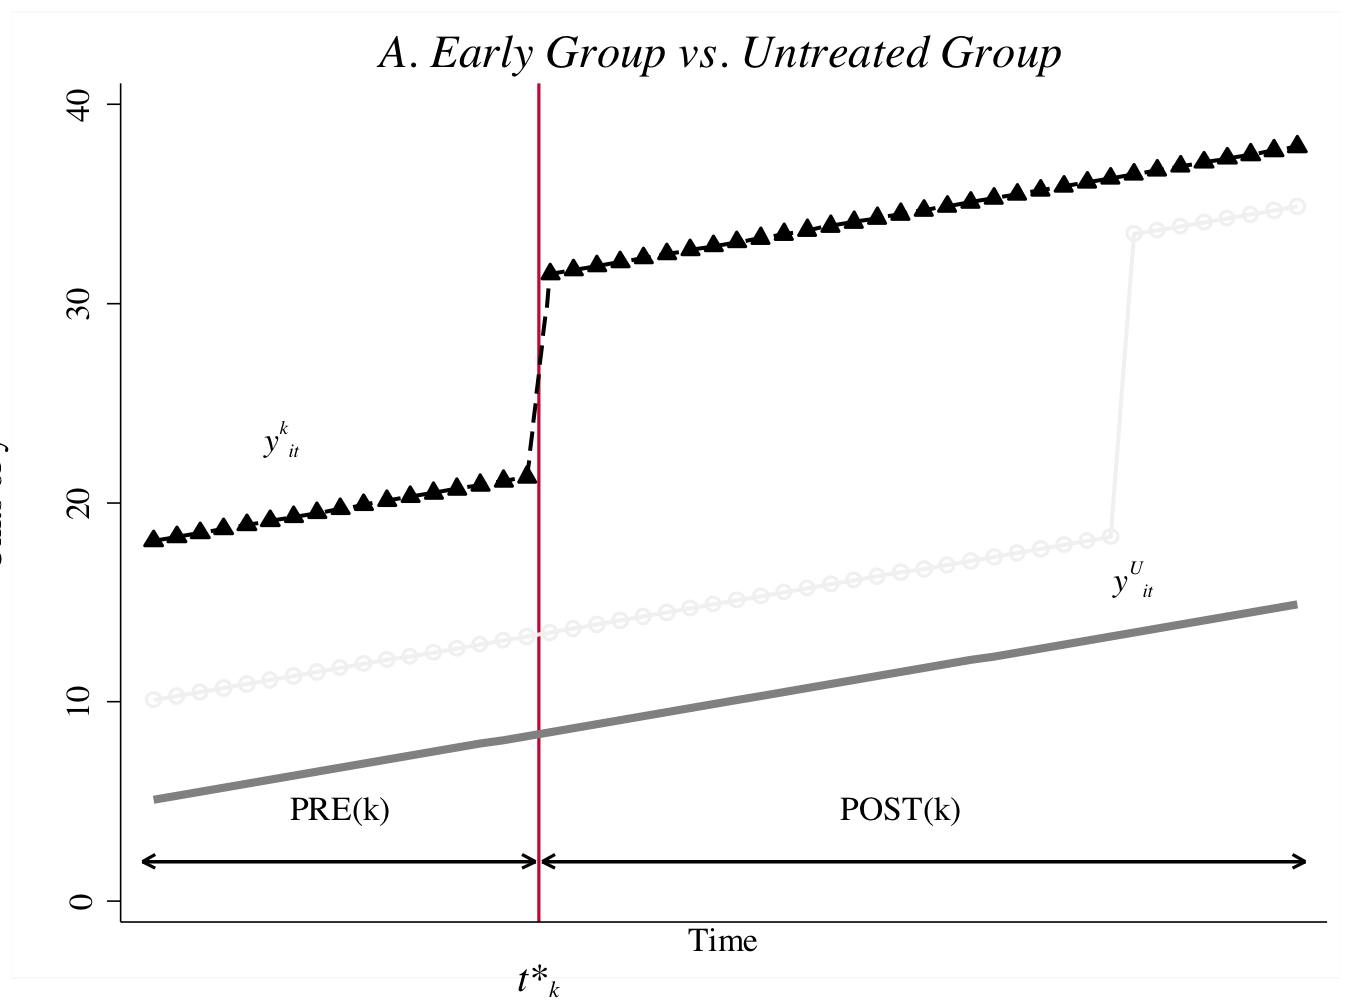
\includegraphics[scale=0.45]{./lecture_includes/bacon_goodman_3.png}
	\end{figure}

\end{frame}

\begin{frame}[plain]
$$\widehat{\delta}^{2x2}_{lU} = \bigg ( \overline{y}_l^{post(l)} - \overline{y}_l^{pre(l)} \bigg ) - \bigg ( \overline{y}_U^{post(l)} - \overline{y}_U^{pre(l)} \bigg ) $$
	\begin{figure}
	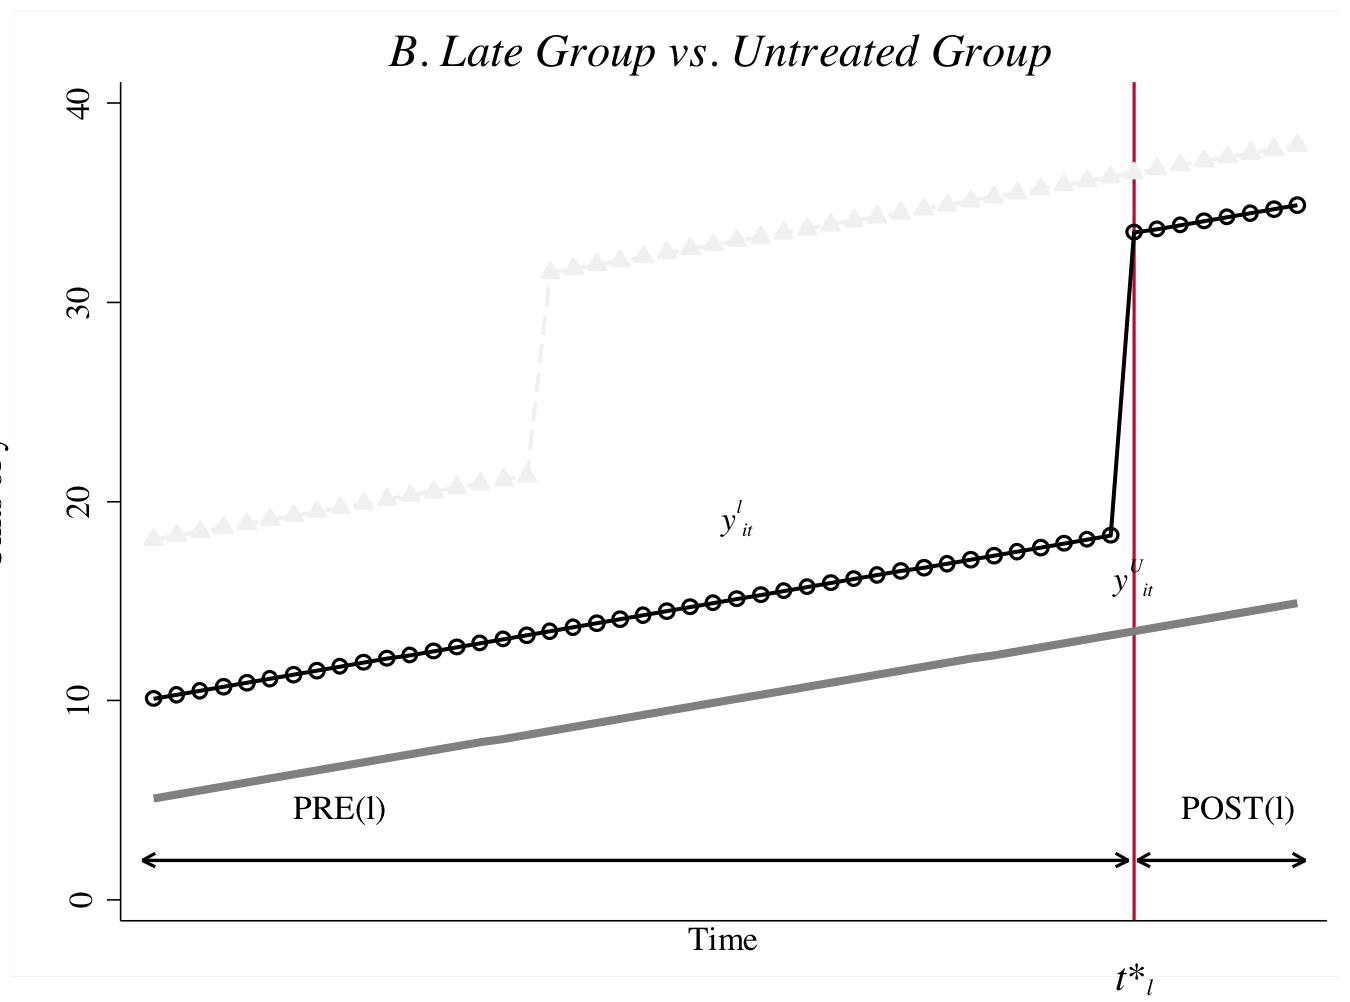
\includegraphics[scale=0.45]{./lecture_includes/bacon_goodman_4.png}
	\end{figure}

\end{frame}


\begin{frame}[plain]

$$\delta_{kl}^{2x2,k} = \bigg ( \overline{y}_k^{MID(k,l)} - \overline{y}_k^{Pre(k,l)} \bigg ) - \bigg ( \overline{y}_l^{MID(k,l)} - \overline{y}_l^{PRE(k,l)} \bigg ) $$

	\begin{figure}
	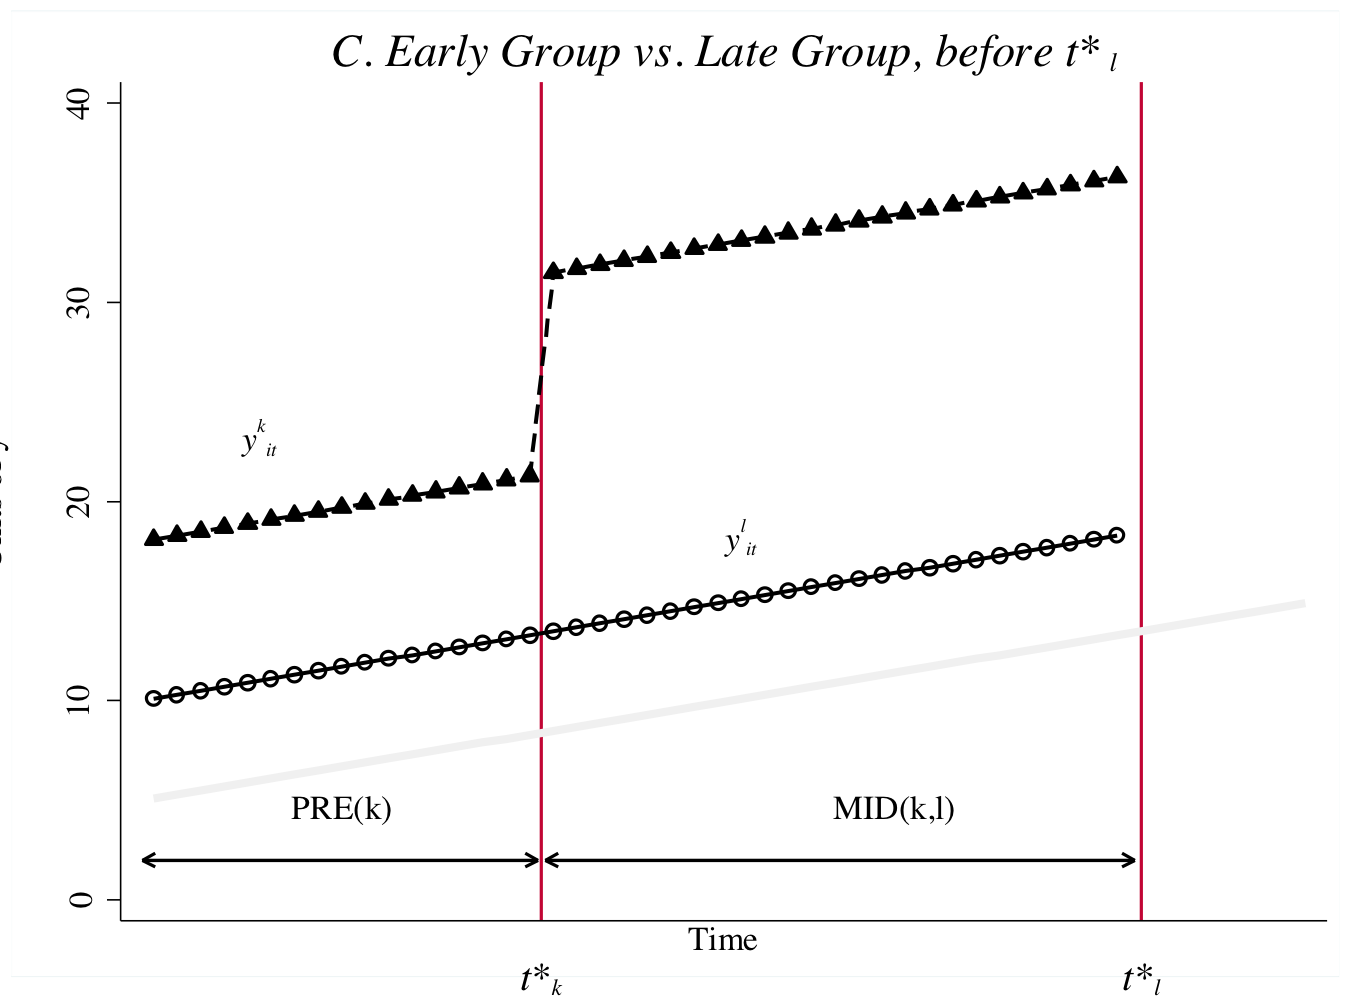
\includegraphics[scale=0.45]{./lecture_includes/bacon_goodman_6.png}
	\end{figure}

\end{frame}

\begin{frame}[plain]
$$\delta_{lk}^{2x2,l} = \bigg ( \overline{y}_l^{POST(k,l)} - \overline{y}_l^{MID(k,l)} \bigg ) - \bigg ( \overline{y}_k^{POST(k,l)} - \overline{y}_k^{MID(k,l)} \bigg ) $$

	\begin{figure}
	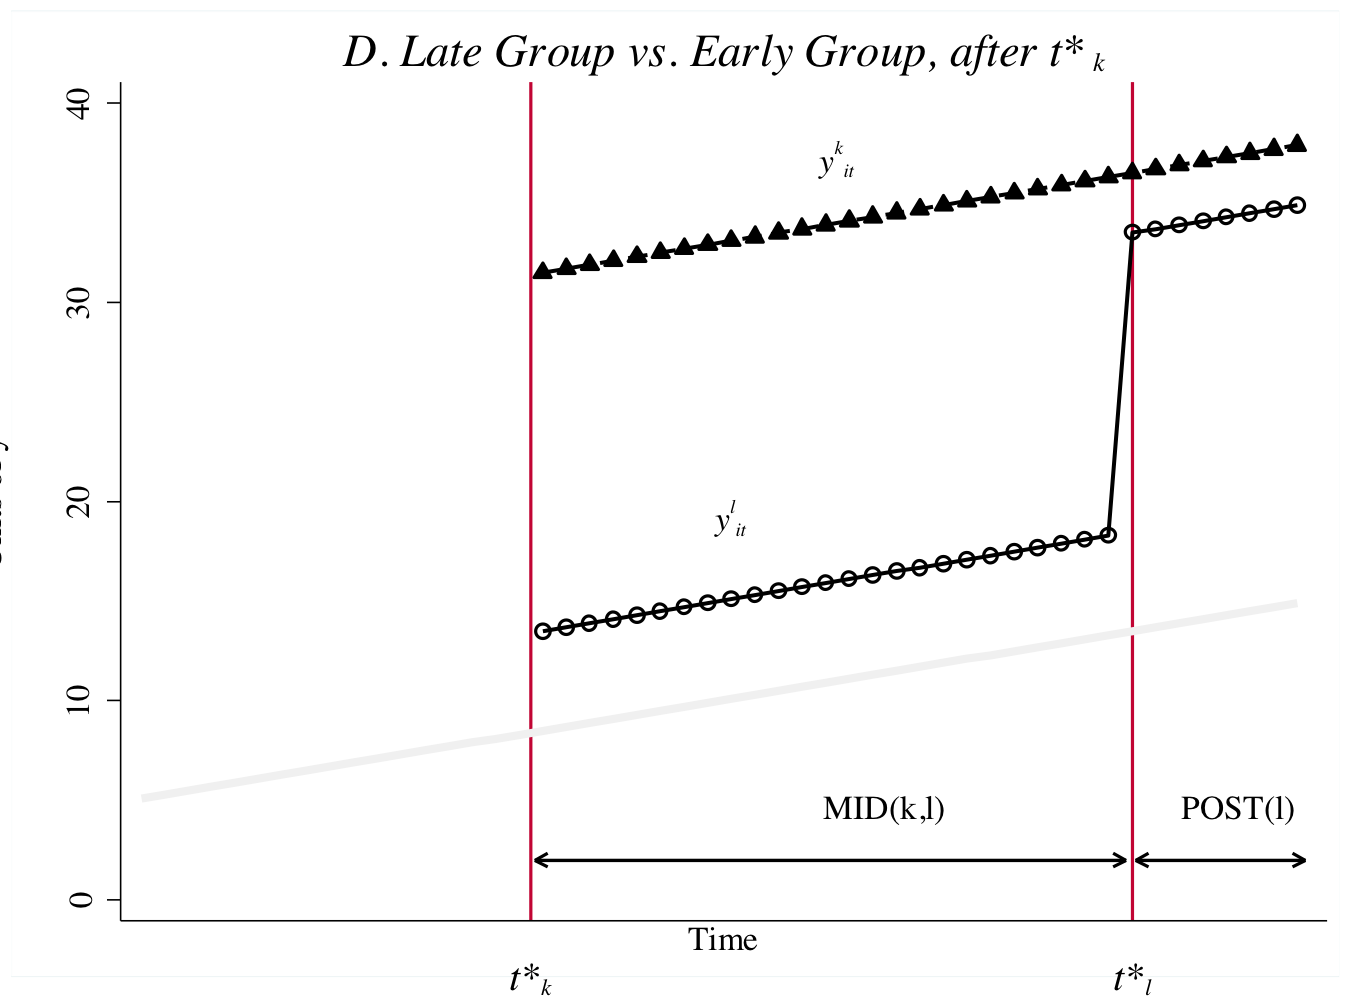
\includegraphics[scale=0.4]{./lecture_includes/bacon_goodman_7.png}
	\end{figure}

\end{frame}


%\begin{frame}[plain]
%\begin{center}
%\textbf{Typical regression equation}
%\end{center}

%$$y_{it}  =  \delta D_{it}  + \alpha_i + \alpha_t + \epsilon_{it}$$

%\begin{enumerate}
%\item Partial out the fixed effects (Frisch-Waugh-Lovell theorem) 
%	\begin{eqnarray*}
%	\tilde{D}_{it} = (D_{it} - \overline{\overline{D}} ) - (\overline{D}_i - \overline{\overline{D}}) - (\overline{D}_t - \overline{\overline{D}} )\\
%	\tilde{y}_{it} = (D_{it} - \overline{\overline{y}} ) - (\overline{y}_i - \overline{\overline{y}}) - (\overline{y}_t - \overline{\overline{y}})
%	\end{eqnarray*}where $\overline{\overline{x}} = \frac{1}{NT}\sum_i \sum_t x_{it}$
%\item Calculate univariate coefficient by brute force
%$$\widehat{\delta}^{DD} = \frac{ \widehat{Cov}(\tilde{D}_{it}, \tilde{y}_{it})}{\widehat{Var}(\tilde{D}_{it})} = \frac{ \frac{1}{NT} \sum_i \sum_t (y_{it} - \overline{\overline{y}})(D_{it} - \overline{\overline{D}})}{ \frac{1}{NT} \sum_i \sum_t (D_{it} - \overline{\overline{D}} ) }$$
%\end{enumerate}

%\end{frame}
	

\begin{frame}{Bacon decomposition}


TWFE estimate yields a weighted combination of each groups' respective 2x2 (of which there are 4 in this example)
\begin{eqnarray*}	
\widehat{\delta}^{DD} = \sum_{k \neq U} s_{kU}\widehat{\delta}_{kU}^{2x2} + \sum_{k \neq U} \sum_{l>k} s_{kl}  \bigg [ \mu_{kl}\widehat{\delta}_{kl}^{2x2,k} + (1-\mu_{kl}) \widehat{\delta}_{lk}^{2x2,l} \bigg]
\end{eqnarray*}where that first 2x2 combines the k compared to U and the l to U (combined to make the equation shorter)

\end{frame}
	


\begin{frame}{Third, the Weights}

 \begin{eqnarray*} s_{ku} &=& \frac{ n_k n_u \overline{D}_k (1- \overline{D}_k ) }{ \widehat{Var} ( \tilde{D}_{it} )} \\
s_{kl} &=& \frac{ n_k n_l (\overline{D}_k - \overline{D}_{l} ) ( 1- ( \overline{D}_k - \overline{D}_{l} )) }{\widehat{Var}(\tilde{D}_{it})} \\
\mu_{kl} &=& \frac{1 - \overline{D}_k }{1 - ( \overline{D}_k - \overline{D}_{l} )}
\end{eqnarray*}where $n$ refer to sample sizes, $\overline{D}_k (1- \overline{D}_k )$ $(\overline{D}_k - \overline{D}_{l} ) ( 1- ( \overline{D}_k - \overline{D}_{l} ))$ expressions refer to variance of treatment, and the final equation is the same for two timing groups.

\end{frame}

\begin{frame}{Weights discussion}

\begin{itemize}
\item Two things to note:
	\begin{itemize}
	\item More units in a group, the bigger its 2x2 weight is
	\item Group treatment variance weights up or down a group's 2x2
	\end{itemize}
\item Think about what causes the treatment variance to be as big as possible. Let's think about the $s_{ku}$ weights.
	\begin{itemize}
	\item $\overline{D}=0.1$. Then $0.1 \times 0.9 = 0.09$
	\item $\overline{D}=0.4$. Then $0.4 \times 0.6 =0.24$
	\item $\overline{D}=0.5$. Then $0.5 \times 0.5 = 0.25$
	\item $\overline{D}=0.6$. Then $0.6 \times 0.4 = 0.24$
	\end{itemize}
\item This means the weight on treatment variance is maximized for \emph{groups treated in middle of the panel}
\end{itemize}
\end{frame}

\begin{frame}{More weights discussion}

\begin{itemize}
\item But what about the ``treated on treated'' weights (i.e., $\overline{D}_k - \overline{D}_{l} $)  
\item Same principle as before - when the difference between treatment variance is close to 0.5, those 2x2s are given the greatest weight
\item For instance, say $t^*_k=0.15$ and $t^*_l=0.67$. Then $\overline{D}_k - \overline{D}_{l} = 0.52$.  And thus $0.52 \times 0.48 = 0.2496$.
\end{itemize}

\end{frame}


\begin{frame}{Summarizing TWFE centralities}

\begin{itemize}
\item Groups in the middle of the panel weight up their respective 2x2s via the variance weighting
\item Decomposition highlights the strange role of panel length when using TWFE
\item Different choices about panel length change both the 2x2 and the weights based on variance of treatment
\end{itemize}

\end{frame}

%\begin{frame}[plain]
%\begin{center}
%\textbf{DD Decomposition Theorem}
%\end{center}

%Assume that there are $k=1,\dots,K$ groups of treated units ordered by treatment time $_k^*$ and one control group $U$ which does not receive treatment in the data.  The share of units in group $k$ is $n_k$ and the share of periods that group $k$ spends under treatment is $\overline{D}_k$. The DD estimate from a two-way fixed effects model is a weighted average of all two-group DD estimators.

%\begin{eqnarray*}
%\widehat{\delta}^{DD} = \sum_{k \neq u} s_{ku} \widehat{\delta}_{ku}^{DD} + \sum_{k \neq u} \sum_{l > k} s_{kl} \bigg [ \mu_{kl} \widehat{\delta}_{kl}^{DD,k} + (1-\mu_{kl} ) \widehat{\delta}_{kl}^{DD,l} \bigg ]
%\end{eqnarray*}with weights equal to  \begin{eqnarray*} s_{ku} &=& \frac{ n_k n_u \overline{D}_k (1- \overline{D}_k ) }{ \widehat{Var} ( \tilde{D}_{it} )} \\
%s_{kl'} &=& \frac{ n_k n_l (\overline{D}_k - \overline{D}_{l} ) ( 1- ( \overline{D}_k - \overline{D}_{l} )) }{\widehat{Var}(\tilde{D}_{it})} \\
%\mu_{kl} &=& \frac{1 - \overline{D}_k }{1 - ( \overline{D}_k - \overline{D}_{j'} )}
%\end{eqnarray*}

%\end{frame}

\begin{frame}{Moving from 2x2s to causal effects and bias terms}

Let's start breaking down these estimators into their corresponding estimation objects expressed in causal effects and biases


\begin{eqnarray*}
\widehat{\delta}^{2x2}_{kU} &=& ATT_k{Post} + \Delta Y^0_k(Post(k),Pre(k)) - \Delta Y^0_U(Post(k),Pre) \\
\widehat{\delta}^{2x2}_{kl} &=& ATT_k(MID) + \Delta Y^0_k(MID,Pre) - \Delta Y^0_l(MID, Pre)
\end{eqnarray*}These look the same because you're always comparing the treated unit with an untreated unit (though in the second case it's just that they haven't been treated \emph{yet}). 

\end{frame}

\begin{frame}{The dangerous 2x2}

But what about the 2x2 that compared the late groups to the already-treated earlier groups? With a lot of substitutions we get:

\begin{eqnarray*}
\widehat{\delta}^{2x2}_{lk} &=& ATT_{l,Post(l)} + \underbrace{\Delta Y^0_l(Post(l),MID) - \Delta Y^0_k ( Post(l), MID)}_{\mathclap{\text{Parallel trends bias}}} \\
&& - \underbrace{(ATT_k(Post) - ATT_k(Mid))}_{\mathclap{\text{Heterogeneity bias!}}}
\end{eqnarray*}


\end{frame}

\begin{frame}{Substitute all this stuff into the decomposition formula}

\begin{eqnarray*}	
\widehat{\delta}^{DD} = \sum_{k \neq U} s_{kU}\widehat{\delta}_{kU}^{2x2} + \sum_{k \neq U} \sum_{l>k} s_{kl}  \bigg [ \mu_{kl}\widehat{\delta}_{kl}^{2x2,k} + (1-\mu_{kl}) \widehat{\delta}_{kl}^{2x2,l} \bigg]
\end{eqnarray*}where we will make these substitutions\begin{eqnarray*}
\widehat{\delta}_{kU}^{2x2} &=& ATT_k(Post) + \Delta Y_l^0(Post,Pre) - \Delta Y_U^0(Post, Pre) \\
\widehat{\delta}_{kl}^{2x2,k} &=& ATT_k(Mid) + \Delta Y_l^0(Mid,Pre) - \Delta Y_l^0(Mid, Pre) \\
\widehat{\delta}^{2x2,l}_{lk} &=& ATT_{l}Post(l) + \Delta Y^0_l(Post(l),MID) - \Delta Y^0_k ( Post(l), MID) \\
&&- (ATT_k(Post) - ATT_k(Mid))
\end{eqnarray*}Notice all those potential sources of biases! 

\end{frame}


\begin{frame}{Potential Outcome Notation}

\begin{eqnarray*}
p\text{ }lim\text{ } \widehat{\delta}^{TWFE}_{n\to\infty} &=& VWATT + VWPT - \Delta ATT
\end{eqnarray*}

\begin{itemize}
\item Notice the number of assumptions needed \emph{even} to estimate this very strange weighted ATT (which is a function of how you drew the panel in the first place). 
\item With dynamics, it attenuates the estimate (bias) and can even reverse sign depending on the magnitudes of what is otherwise effects in the sign in a reinforcing direction! 
\item Let's look at each of these three parts more closely
\end{itemize}

\end{frame}


\begin{frame}{Variance weighted ATT}

\begin{eqnarray*}
VWATT &=& \sum_{k \neq U} \sigma_{kU} ATT_k(Post(k))\\
&+& \sum_{k \neq U} \sum_{l>k} \sigma_{kl} \bigg [ \mu_{kl} ATT_k (MID)+ (1-\mu_{kl}) ATT_{l} (POST(l)) \bigg ]
\end{eqnarray*}where $\sigma$ is like $s$ only population terms not samples.  
\begin{itemize}
\item Weights sum to one. 
\item Note, if all the ATT are identical, then the weighting is irrelevant. 
\item But otherwise, it's basically weighting each of the individual sets of ATT we have been discussing, where weights depend on group size and variance
\end{itemize}

\end{frame}

\begin{frame}{Variance weighted parallel trends}

\begin{eqnarray*}
VWPT &=& \sum_{k \neq U} \sigma_{kU} \bigg [ \Delta Y_k^0(Post(k),Pre) - \Delta Y_U^0(Post(k),Pre) \bigg ] \\
&+& \sum_{k \neq U} \sum_{l>k} \sigma_{kl} \bigg [ \mu_{kl} \{ \Delta Y^0_k(Mid,Pre(k)) - \Delta Y_l^0(Mid,Pre(k))\} \\
&+&(1-\mu_{kl}) \{ \Delta Y^0_l(Post(l), Mid) - \Delta Y^0_k(Post(l), Mid) \} \bigg ]
\end{eqnarray*}There are $K^2$ parallel trends inside the weights. Their weighted average must equal zero.

\end{frame}

\begin{frame}{Heterogeneity bias}

\begin{eqnarray*}
\Delta ATT = \sum_{k \neq U} \sum_{l>k} (1 - \mu_{kl}) \bigg [ ATT_k(Post(l) - ATT_k(Mid)) \bigg ]
\end{eqnarray*}Now, if the ATT is constant over time, then this difference is zero, but what if the ATT is not constant? Then TWFE is biased, and depending on the dynamics and the VWATT, may even flip signs
\end{frame}

\subsection{Castle doctrine reform}


\begin{frame}[plain]
	\begin{figure}
	
\includegraphics[scale=0.5]{./lecture_includes/cheng_and_hoekstra_jhr.png}
	\end{figure}

\end{frame}

\begin{frame}{Case study: Castle doctrine reforms}

\begin{itemize}

\item Cheng and Hoekstra (2013) is a good, clean example of a differential timing for us to practice on
\item In 2005, Florida passed a law called Stand Your Ground that expanded self-defense protections beyond the house
\item More ``castle doctrine'' reforms followed from 2006 to 2009

\end{itemize}

\end{frame}

\begin{frame}{Description}

Details of castle doctrine reforms
		\begin{itemize}
		\item ``Duty to retreat'' is removed versus castle doctrine reforms; expanded where you can use lethal force
		\item Presumption of reasonable fear is added
		\item Civil liability for those acting under the law is removed
		\end{itemize}
\end{frame}

\begin{frame}{Ambiguous predictions}
	
Castle reforms $\rightarrow$ homicides: Increase by removing homicide penalties and increasing opportunities
	\begin{itemize}
	\item Castle doctrine expansions lowered the (expected) cost of killing someone in self-defense
	\item Lowering the price of lethal self-defense should increase lethal homicides
	\end{itemize}
\bigskip
Castle reforms $\rightarrow$ homicides: decrease through deterrence

\end{frame}


\begin{frame}{Cheng and Hoekstra's estimation model}
	
	\begin{itemize}
	\item TWFE model$$Y_{it} = \beta_1 D_i + \beta_2 T_t + \beta_3 (CDL_{it}) + \alpha_1X_{it} + c_i + u_t + \varepsilon_{it}$$
	\item $CDL$ is a fraction between 0 and 1 depending on the percent of the year the state has a castle doctrine law 
	\item Preferred specifications includes ``region-by-year fixed effects'' (see next slide)
	\item Estimation with TWFE and Poisson with and without population weights
	\item Models will include covariates (e.g., police, imprisonment, race shares, state spending on public assistance)
	\end{itemize}
\end{frame}


\begin{frame}{Publicly available crime data}
	
Main data: FBI Uniform Crime Reports Part 1 Offenses (2000-2010)
		\begin{itemize}
		\item Main outcomes: log homicides
		\item Falsification outcomes: motor vehicle theft and larceny
		\item Deterrence outcomes: burglary, robbery, assault
		\end{itemize}
\end{frame}



\begin{frame}{Region-by-year fixed effects}
	
	\begin{itemize}
	\item \textbf{Parallel trends assumption}: imposed structurally with region-by-year dummies
	\item \textbf{Argument}: unobserved changes in crime are running ``parallel'' to the treatment states within region over time
	\item \textbf{SUTVA} and \textbf{No Anticipation}: No spillovers, no hidden variation in treatment, no behavioral change today in response to tomorrow's law
	\end{itemize}
\end{frame}



\begin{frame}{Results -- Deterrence}
	
	\begin{figure}
	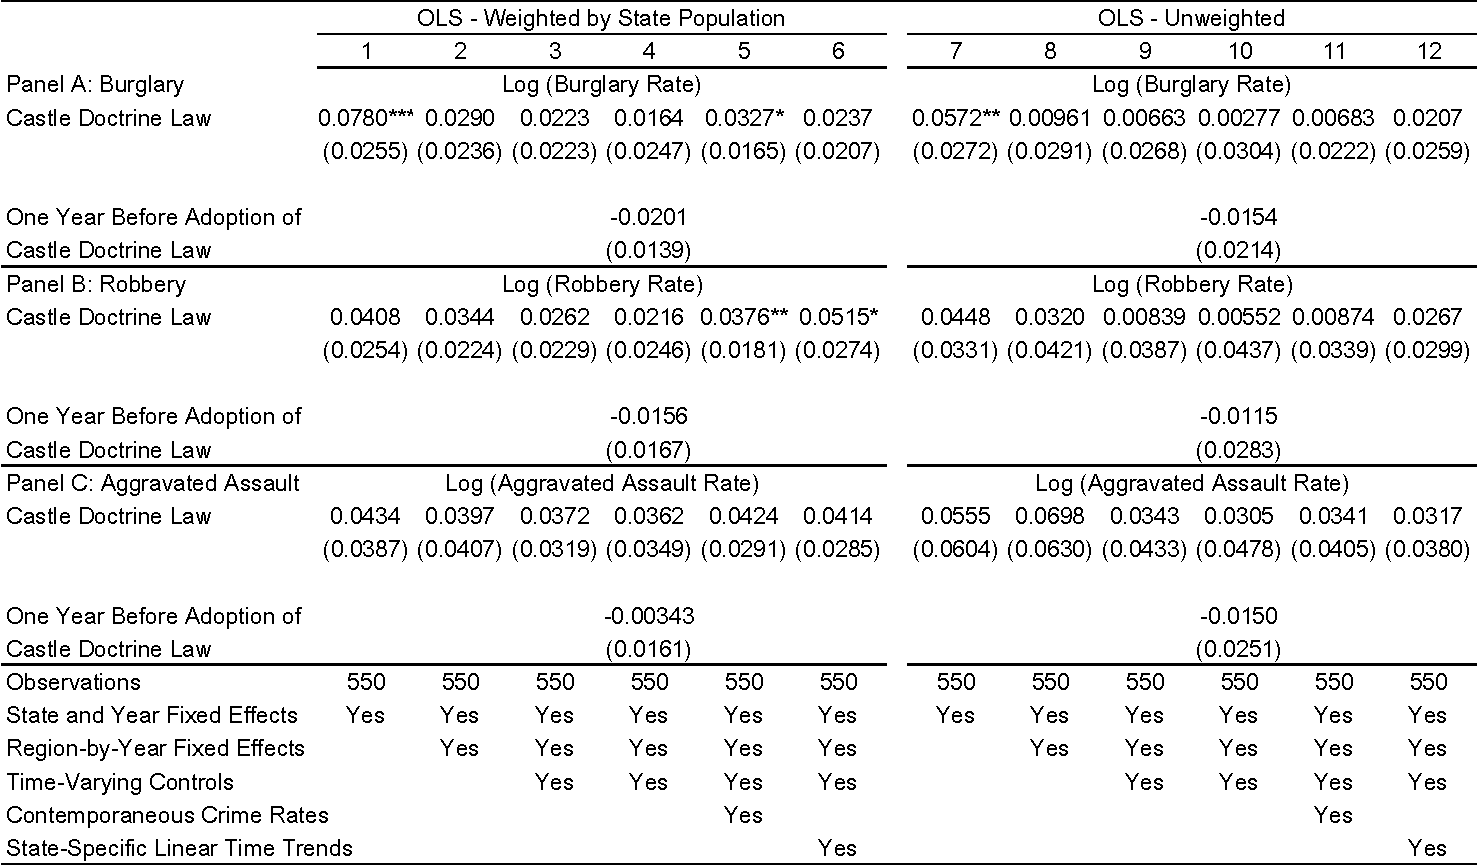
\includegraphics[scale=0.4]{./lecture_includes/cheng4.pdf}
	\end{figure}
\end{frame}




\begin{frame}{Results -- Homicides}
	
	\begin{figure}
	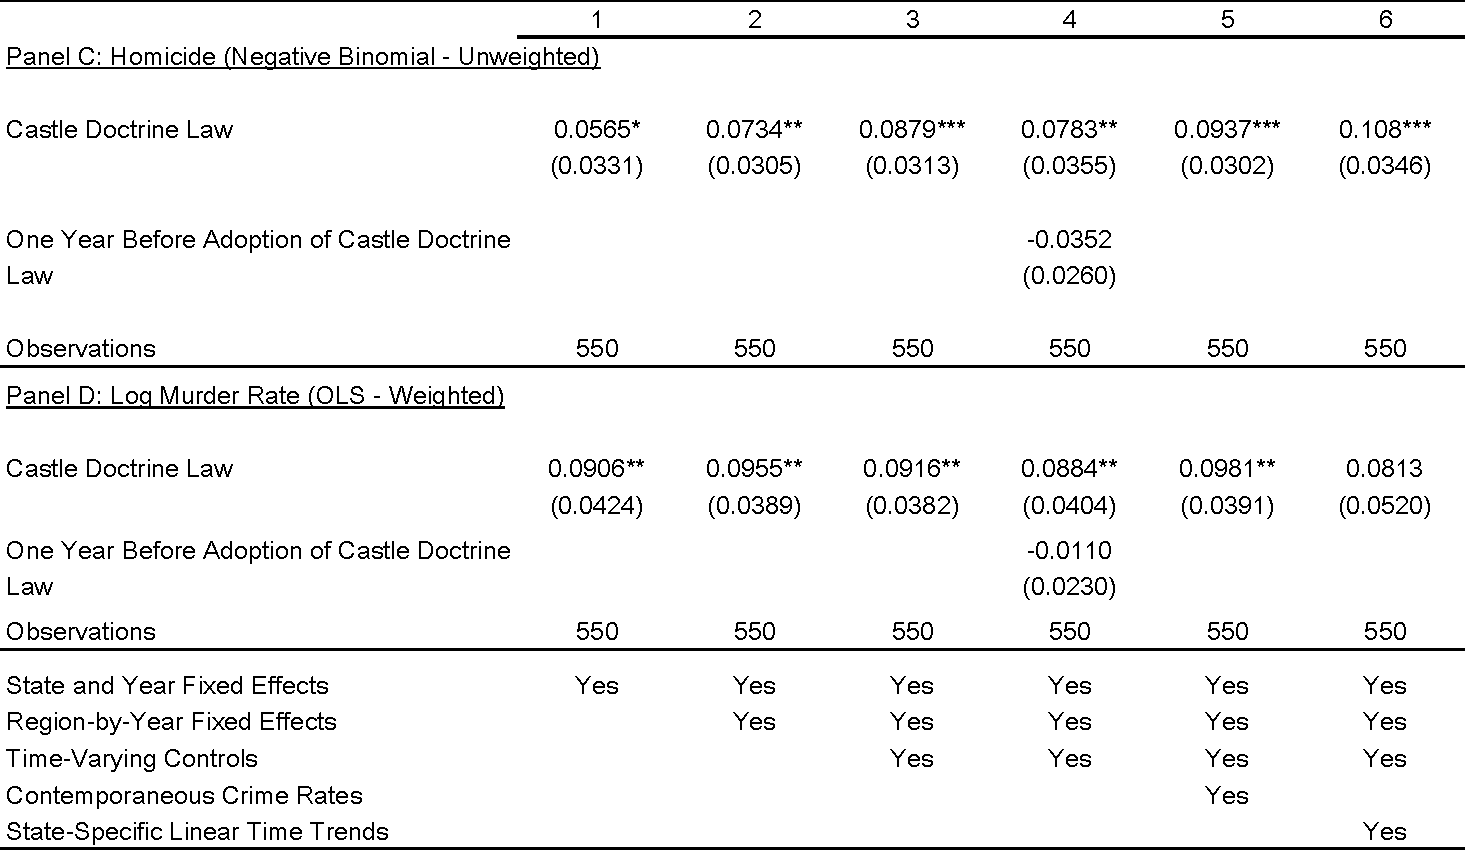
\includegraphics[scale=0.4]{./lecture_includes/cheng12.pdf}
	\end{figure}
\end{frame}



\begin{frame}{Interpretation}
	
	\begin{itemize}
	\item Series of robustness checks (falsifications on larceny and motor vehicle theft; deterrence; many different specifications)
	\item Castle doctrine reforms are associated with an 8\% net increase in homicide rates per year across the 21 adopting states
	\item Interpretation is these would not have occurred without castle doctrine reforms
	\item But is this robust to alternative models? Today we will check
	\end{itemize}
\end{frame}




\section{Implicit imputation}

\subsection{CS}

\begin{frame}{Imbens and Rubin 2015}

\begin{quote}
``At some level, all methods for causal inference can be viewed as imputation methods, although some more explicitly than others.'' -- Imbens and Rubin (2015)
\end{quote}

\end{frame}


\begin{frame}{Causal inference involves imputation}

\begin{itemize}
\item Causal inference is a missing data problem -- we are missing counterfactuals
\item Recall that estimating the ATT necessarily involved correctly imputing the counterfactual using parallel trends
\item OLS, therefore, is \emph{implicitly} imputing counterfactuals for estimating the ATT
\item We'll review a few studies that do this
\end{itemize}

\end{frame}



\begin{frame}{Callaway and Sant'Anna 2020}

\begin{itemize}
\item New papers are coming out focused on the issues that we are seeing with TWFE
\item I'll discuss one though by Callaway and Sant'anna (2020) due to time constraints (call it CS)
\item If we have time, I'll run through a simulation illustrating both the bias of TWFE and the unbiased estimation of this CS estimator
\item Interesting ancestry -- CS is a descendent of Abadie (2005) from earlier

\end{itemize}

\end{frame}

\begin{frame}{Preliminary}

CS considers identification, aggregation, estimation and inference procedures for ATT in DD designs with

\begin{enumerate}
\item multiple time periods
\item variation in treatment timing (i.e., differential timing)
\item parallel trends only holds after conditioning on observables
\end{enumerate}

\end{frame}

\begin{frame}{When might you use this estimator}

Probably in the very situations describing your own study
\begin{enumerate}
\item When treatment effects heterogenous by time of adoption
\item When treatment effects change over time
\item When shortrun effects more pronounced than longrun effects
\item When treatment effect dynamics differ if people are first treated in a recession relative to expansion years
\end{enumerate}

\end{frame}





\begin{frame}{Group-time ATT is the parameter of interest in CS}

\begin{eqnarray*}
ATT(g,t) = E[Y_t^1 - Y_t^0 | G_g=1]
\end{eqnarray*}

\end{frame}


\begin{frame}{Group-time ATT}

Group-time ATT is the ATT for a specific group and time
\begin{itemize}
\item Groups are basically cohorts of units treated at the same time
\item CS will calculate an ATT per group/time which will be the sum of all $T-t_k$ for all groups (i.e., a lot)
\item Group-time ATT estimates are not determined by the estimation method one adopts (first difference or FE) bc they are simple differences in means
\item Does not directly restrict heterogeneity with respect to observed covariates, timing or the evolution of treatment effects over time
\item Provides a way to aggregate over these to get a single ATT
\item Inference is the bootstrap
\end{itemize}

\end{frame}



\begin{frame}{Notation}

\begin{itemize}
\item $T$ periods going from $t=1, \dots, T$
\item Units are either treated ($D_t=1$) or untreated ($D_t=0$) but once treated cannot revert to untreated state
\item $G_g$ signifies a group and is binary.  Equals one if individual units are treated at time period $t$.
\item $C$ is also binary and indicates a control group unit equalling one if ``never treated'' (can be relaxed though to ``not yet treated'')
	\begin{itemize}
	\item Recall the problem with TWFE on using treatment units as controls
	\end{itemize}
\item Generalized propensity score enters into the estimator as a weight: $$\widehat{p(X)} = Pr(G_g=1 | X,G_c+C=1)$$
\end{itemize}

\end{frame}

\begin{frame}{Assumptions}

Assumption 1: Sampling is iid (panel data) \\
\bigskip
Assumption 2: Conditional parallel trends (for either never treated or not yet treated) \\
\begin{eqnarray*}
E[Y_t^0 - Y_{t-1}^0 | X,G_g=1] = [Y_t^0 - Y_{t-1}^0 | X,C=1] 
\end{eqnarray*}
\bigskip
Assumption 3: Irreversible treatment \\
Assumption 4: Common support (propensity score) \\
\bigskip
Assumption 5: Limited treatment anticipation (i.e., treatment effects are zero pre-treatment)

\end{frame}

\begin{frame}{CS Estimator (the IPW version)}

\begin{eqnarray*}
ATT(g,t) = E \bigg [ \bigg ( \frac{G_g}{E[G_g]} - \frac{ \frac{\hat{p}(X)C}{1-\hat{p}(X)}}{E \bigg [ \frac{\hat{p}(X)C}{1-\hat{p}(X)} \bigg ]} \bigg ) (Y_t - Y_{g-1} ) \bigg ) \bigg ]
\end{eqnarray*}

This is the inverse probability weighting estimator.  Alternatively, there is an outcome regression approach and a doubly robust. Sant'Anna recommends DR. Notice hw CS doesn't use already-treated as controls.
\end{frame}



\begin{frame}{Staggered adoption (i.e., universal coverage)}


\begin{proof}{\textbf{Remark 1:}}
In some applications, eventually all units are treated, implying that $C$ is never equal to one. In such cases one can consider the ``not yet treated'' ($D_t = 0$) as a control group instead of
the ``never treated?'' ($C = 1$).
\end{proof}

\end{frame}

\begin{frame}{Aggregated vs single year/group ATT}

\begin{itemize}
\item The method they propose is really just identifying very narrow ATT per group time.
\item But we are often interested in  more aggregate parameters, like the ATT across all groups and all times
\item They present two alternative methods for building ``interesting parameters'' 
\item Inference from a bootstrap
\end{itemize}


\end{frame}



\begin{frame}{Stata simulation}

Let's now review a simulation in Stata which can be downloaded from my github repo called \texttt{baker.do}.  

\bigskip

\end{frame}




\subsection{SA}


\begin{frame}{Pre-trends}

\begin{itemize}

	\item The identifying assumption for all DD designs is parallel trends
	\item Parallel trends cannot be directly verified because technically one of the parallel trends is an unobserved counterfactual
	\item But one often will check a hunch for parallel trends using pre-trends
	\item But, even if pre-trends are the same one still has to worry about other policies changing at the same time (omitted variable bias)

\end{itemize}

\end{frame}

\begin{frame}{Plot the raw data when there's only two groups}

	\begin{figure}
	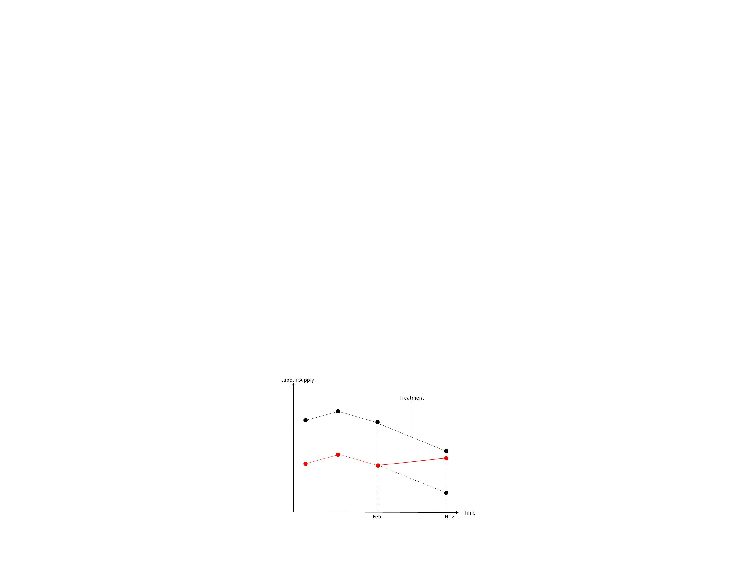
\includegraphics[scale=2.5]{./lecture_includes/waldinger_dd_6.pdf}
	\end{figure}

\end{frame}



\begin{frame}{Event study regression}
	
	\begin{itemize}
	\item Including leads into the DD model is an easy way to analyze pre-treatment trends
	\item Lags can be included to analyze whether the treatment effect changes over time after assignment
	\item The estimated regression would be:$$Y_{its} = \gamma_s + \lambda_t + \sum_{\tau=-2}^{-q}\gamma_{\tau}D_{s\tau} + \sum_{\tau=0}^m\delta_{\tau}D_{s\tau}+\varepsilon_{ist}$$
		\begin{itemize}
		\item Treatment occurs in year 0
		\item Includes $q$ leads or anticipatory effects
		\item Includes $m$ leads or post treatment effects
		\end{itemize}
	\end{itemize}
\end{frame}


\begin{frame}{Medicaid and Affordable Care Act example}

\begin{itemize}
\item Miller, et al. (2019) examine a rollout of Medicaid under the Affordable Care Act
\item They link large-scale survey data with administrative death records
\item 9.3 reduction in annual mortality caused by Medicaid expansion
\item Driven by a reduction in disease-related deaths which grows over time
\end{itemize}

\end{frame}

\imageframe{./lecture_includes/Miller_Medicaid1.png}

\imageframe{./lecture_includes/Miller_Medicaid2.png}

\imageframe{./lecture_includes/Miller_Medicaid3.png}


\begin{frame}[plain]

	\begin{figure}
	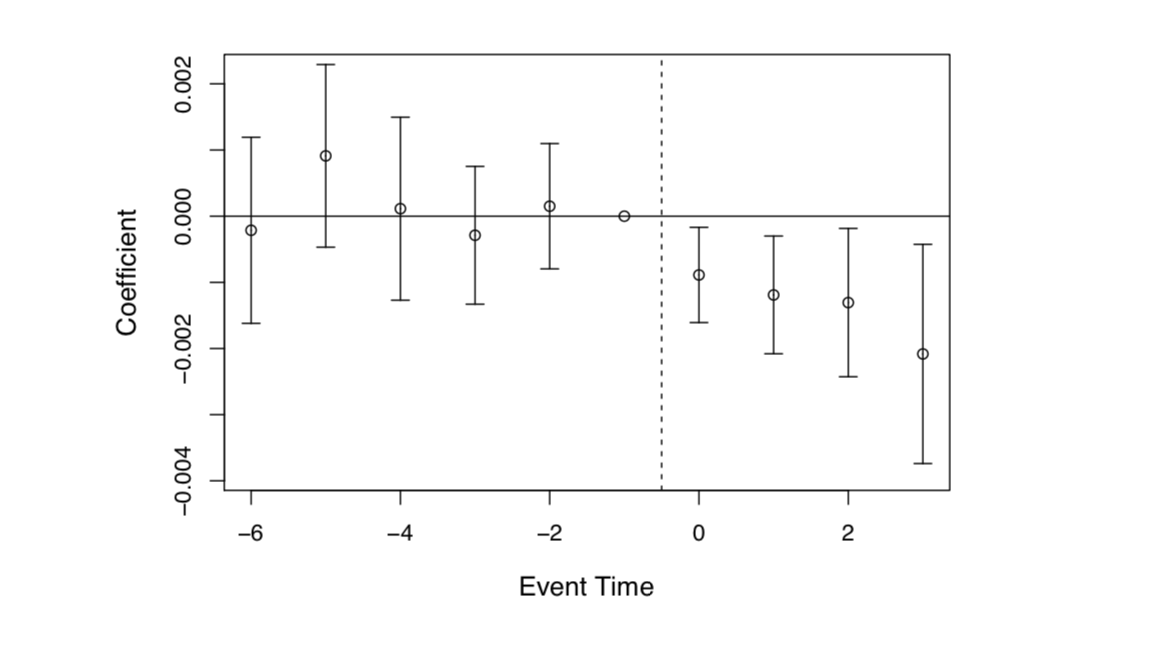
\includegraphics[scale=0.3]{./lecture_includes/Miller_Medicaid4.png}
	\caption{Miller, et al. (2019) estimates of Medicaid expansion's effects on on annual mortality}
	\end{figure}

\end{frame}


\begin{frame}{Differential timing complicates plotting sample averages}

\begin{itemize}
\item New Jersey treated in late 1992, New York in late 1993, Pennsylvania never treated
\item Pre-treatment:
	\begin{itemize}
	\item New Jersey: $<$1992
	\item New York: $<$1993
	\item Pennsylvania: undefined
	\end{itemize}
\item So how do we check parallel leads?

\end{itemize}

\end{frame}

\begin{frame}{Early efforts at event studies}

	\begin{figure}
	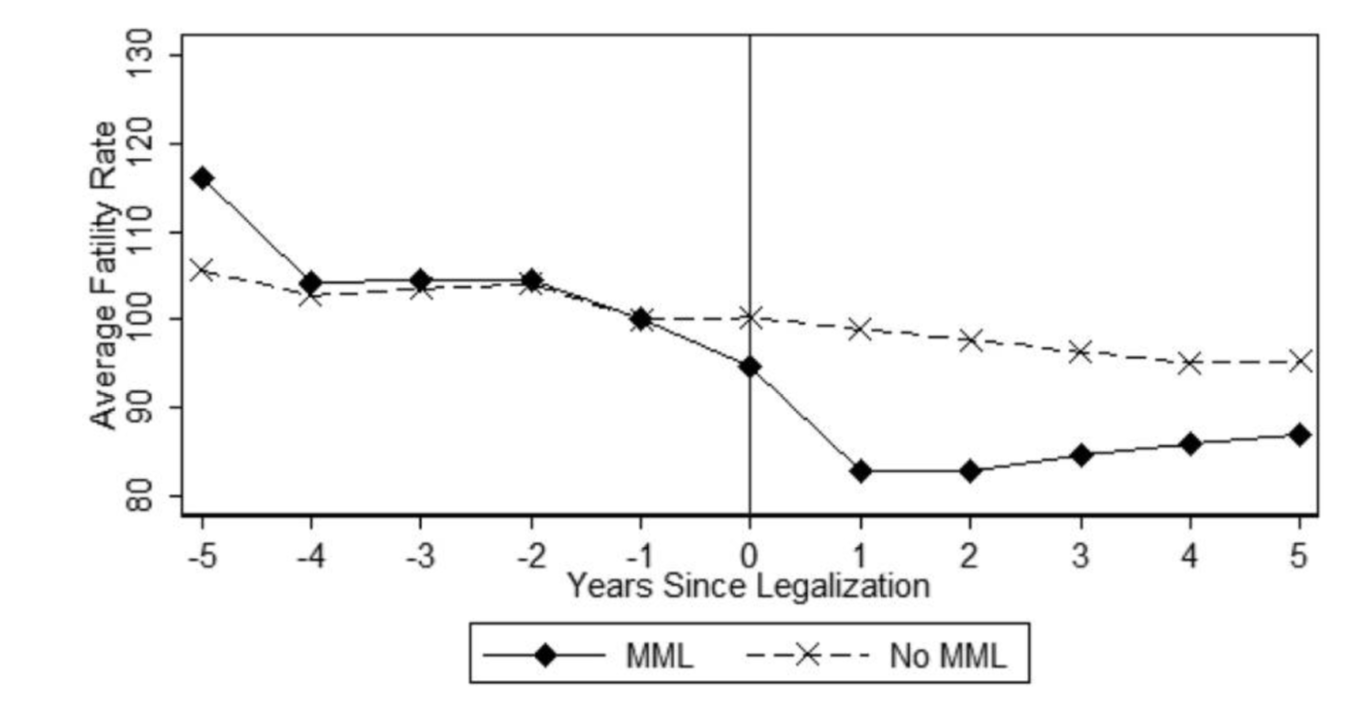
\includegraphics[scale=0.25]{./lecture_includes/mml_eventstudy.png}
	\caption{Anderson, et al. (2013) display of raw traffic fatality rates for re-centered treatment states and control states with randomized treatment dates}
	\end{figure}

\end{frame}

\begin{frame}{Randomized control counties to receive arbitrary dates as treatment can be misleading}

	\begin{figure}
	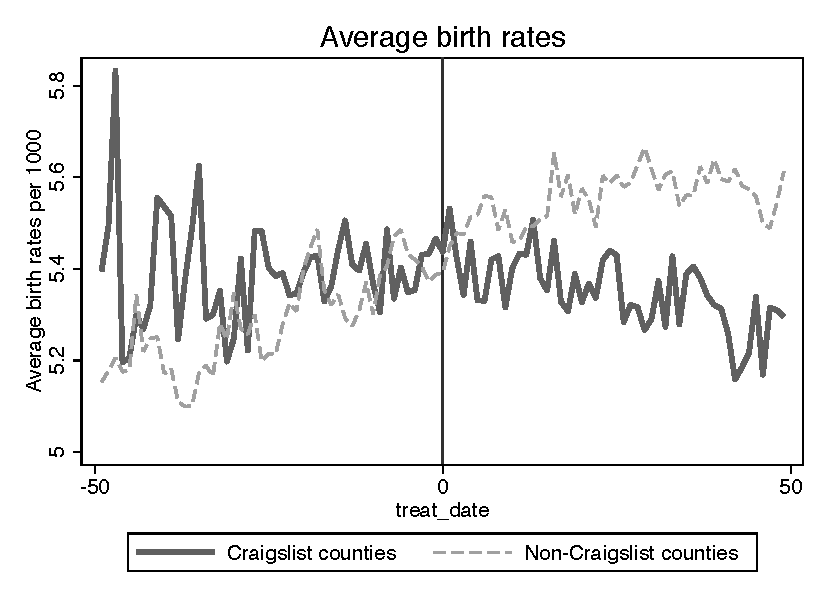
\includegraphics[scale=0.5]{./lecture_includes/dd.pdf}
	\caption{From one of my studies. Looks decent right?}
	\end{figure}

\end{frame}



\begin{frame}[plain]
	\begin{figure}
	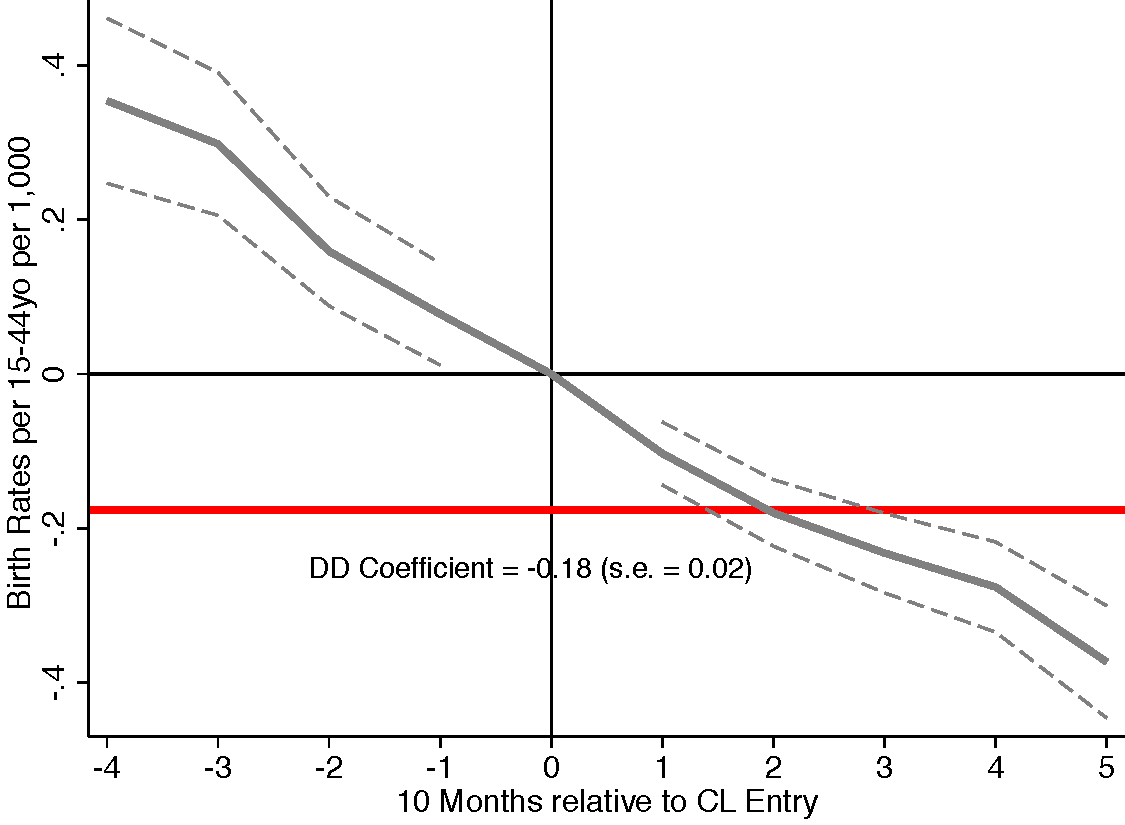
\includegraphics[scale=0.5]{./lecture_includes/br1544.pdf}
	\end{figure}
	
Same data as a couple slides ago, leads don't look good
	
\end{frame}



\begin{frame}{Sun and Abraham 2020}

\begin{itemize}
\item Recall our discussion of event studies estimated with TWFE under differential timing
\item Now that we know about the biases of TWFE when estimating aggregate DD parameters, let's revisit event studies under differential timing
\item Callaway and Sant'Anna (2020) propose alternative estimators for event studies that estimate group-time ATT in relative event time
\item But now we will discuss Sun and Abraham (2020) [SA] which is like a blend of Goodman-Bacon's decomposition and Callaway and Sant'anna alternative estimator to TWFE
\end{itemize}

\end{frame}

\begin{frame}{Summarizing}

\begin{itemize}
\item Goodman-Bacon (2021, forthcoming) focused on decomposition of TWFE to show bias under differential timing
\item Callaway and Sant'anna (2020) presents alternative estimator that yields unbiased estimates of group-time ATTs which can be aggregated or put into event study plots
\item Sun and Abraham (SA) is like a combination of the two papers
\end{itemize}

\end{frame}


\begin{frame}{Summarizing (cont.)}

	\begin{enumerate}
	\item SA is a decomposition of the population regression coefficient on event study leads and lags with differential timing estimated with TWFE
	\item They show that the population regression coefficient is ``contaminated'' by information from other leads and lags
	\item SA presents an alternative estimator that is not so dissimilar to CS
	\end{enumerate}

\end{frame}

\begin{frame}{Summarizing (cont.)}

\begin{itemize}
\item Problems seem to occur with DD when we introduce treatment effect heterogeneity
%\item Leads and lags in the event study estimated with TWFE are contaminated by treatment effects, oddly enough, from other relative periods
\item Under treatment effect heterogeneity, spurious non-zero positive lead coefficients even when there is no pretrend
\item This problem is exacerbated by the TWFE related weights as under some scenarios, the weights sum to zero and``cancel out'' the treatment effects from other periods 
\item They present a 3-step TWFE based alternative estimator which addresses the problems that they find
\end{itemize}

\end{frame}

\begin{frame}{Summarizing (cont.)}

\begin{itemize}
\item Only decomposition of TWFE estimating dynamic leads and lags (Goodman-Bacon focused on a ``static'' specification)
\item Contamination of coefficients on leads and lags by treatment effects depends on the magnitude of the weights on the true group-time ATT, or ``cohort-specific ATT''
\item Weights are a function of cohort composition
\item Examining weights lets you gauge how treatment effect heterogeneity would interact with potential non-zero and non-convex weighting in population regression coefficients on the leads and lags
\end{itemize}

\end{frame}


\begin{frame}{Difficult notation sadly}

\begin{itemize}
\item When treatment occurs at the same time, we say they are part of the same cohort, $e$
\item If we bin the data, then a lead or lag $l$ will appear in the bin $g$ so sometimes they use $g$ instead of $l$ or $l \in g$
\item Building block is the ``cohort-specific ATT'' or $CATT_{e,l}$ -- same thing as CS group-time ATT
\item Estimate $CATT_{e,l}$ with population regression coefficient $\mu_l$
\end{itemize}

\end{frame}


\begin{frame}{Difficult notation (cont.)}

\begin{itemize}
\item At each time $t$ there are two possible treatment status $D_{i,t} \in \{0,1\}$ over $T+1$ time periods
\item Path of treatment status scales exponentially with $T$ and  an take on $2^{T+1}$ possible values
\item They focus on irreversible treatment where treatment status is non-decreasing sequence of zeroes and ones
\end{itemize}

\end{frame}

\begin{frame}{Difficult notation (cont.)}

\begin{itemize}
\item If a group is never treated, the $\infty$ symbol is used to either describe the group ($E_i=\infty$) or the potential outcome ($Y^{\infty}$)
\item $Y^{\infty}_{i,t}$ is is the potential outcome for unit $i$ if it had never received treatment (versus received it later), also called the baseline outcome
\item Other counterfactuals are possible -- maybe unit $i$ isn't ``never treated'' but treated later in counterfactual
\end{itemize}
\end{frame}

\begin{frame}{More difficult notation (cont.)}

\begin{itemize}
\item Treatment effects are the difference between the observed outcome relative to the never-treated counterfactual outcome: $Y_{i,t} - Y^{\infty}_{i,t}$
\item We can take the average of treatment effects at a given relative time period across units first treated at time $E_i=e$ (same cohort) which is what we mean by $CATT_{e,l}$
\item Doesn't use $t$ index time (``calendar time''), rather uses $l$ which is time until or time after treatment date $e$ (``relative time'')
\item Think of it as ${l}=$year - treatment date
\end{itemize}

\end{frame}

\begin{frame}{Definition 1}

\textbf{Definition 1:} The cohort-specific ATT $l$ periods from initial treatment date $e$ is:

\begin{eqnarray*}
CATT_{e,l} = E[Y_{i,e+l} - Y^{\infty}_{i,e+l} | E_i=e]
\end{eqnarray*}

\end{frame}


\begin{frame}{Identifying assumption 1}

\textbf{Assumption 1: Parallel trends in baseline outcomes}: $E[Y^{\infty}_{i,t} - Y^{\infty}_{i,s} | E_i = e ]$ is the same for all $e \in supp(E_i)$ and for all $s$, $t$ and is equal to $E[Y^{\infty}_{i,t} - Y^{\infty}_{i,s} ]$

\bigskip

Interesting SA comment: Never-treated units are likely to differ from ever-treated units in many ways; think of a Roy model.  What does it imply that they chose not to get treated? It may imply net negative treatment effects and that could mean they may not share the same evolution of baseline outcomes as the treatment groups. If you think they are unlikely to satisfy this assumption, then drop them.  Almost like a synthetic control approach.

\end{frame}


\begin{frame}{Assumption 2}

\textbf{Assumption 2: No anticipator behavior in pre-treatment periods}: There is a set of pre-treatment periods such that $E[Y_{i,e+l}^e - Y_{i,e+l}^{\infty} | E_i = e]=0$ for all possible leads.

\bigskip

Basically means that potential outcomes prior to treatment at baseline by on average the same.  This means there is no pre-trends, essentially.  This is most plausible if the full treatment paths are not known to the units (e.g., Craigslist opening erotic services without announcement)

\end{frame}


\begin{frame}{Assumption 3}

\textbf{Assumption 3: Treatment effect homogeneity}: For each relative time period $l$, the $CATT_{e,l}$ doesn't depend on the cohort and is equal to $CATT_l$. 

\bigskip

Assumption 3 requires each cohort experience the same path of treatment effects. Treatment effects need to be the same across cohorts in every relative period for homogeneity to hold, whereas for heterogeneity to occur, treatment effects just need to differ across cohorts in one relative time period.  Doesn't preclude dynamic treatment effects, though.  It just imposes that cohorts share the same treatment path.

\end{frame}

\begin{frame}{Treatment effect heterogeneity}

\begin{itemize}
\item Assumption 3 is violated when different cohorts experience different paths of treatment effects
\item Cohorts may differ in their covariates which affect how they respond to treatment (e.g., if treatment effects vary with age, and there is variation in age across units first treated at different times, then there will be heterogeneous treatment effects)
\item Doesn't rule out parallel trends
\end{itemize}

\end{frame}

\begin{frame}{TWFE Regression}

\begin{eqnarray*}
Y_{i,t} = \alpha_i + \delta_t + \sum_{g \in G} \mu_g1\{t-E_i \in g \} + \varepsilon_{i,t}
\end{eqnarray*}


\bigskip

They say $E_i$ is the initial time of a binary variable absorbing treatment for unit $i$. Fixed effects should be obvious.  $\mu_g$ is the population regression coefficient on the leads and lags that we want to estimate. We estimate this using OLS and get $\widehat{\mu_g}$. 

\bigskip

We are interested in the properties of $\mu_g$ under differential timing as well as whether there are any never-treated units

\end{frame}


\begin{frame}{Specifying the leads and lags}

How will we specify the $1\{t-E_i \in g \} $ term?  SA considers a couple:

\begin{enumerate}
\item Static specification: $$Y_{i,t} = \alpha_i + \delta_t + \mu_g \sum_{l \geq 0}D^l_{i,t} + \varepsilon_{i,t}$$
\item Dynamic specification: $$Y_{i,t} = \alpha_i + \delta_t + \sum_{l = -K}^{-2} \mu_l D^l_{i,t} + \sum_{l=0}^L\mu_lD^l_{i,t}+ \varepsilon_{i,t}$$
\end{enumerate}


\end{frame}


\begin{frame}{Multicollinearity}

Dynamic specification requires deciding which leads to drop.  They recommend dropping two: $l=-1$ and some other one (they seem to favor $l=-4$).  The reason is twofold. You drop one of them to avoid multicollinearity in the relative time indicators. You drop a second one because of the multicollinearity coming from the linear relationship between TWFE and the relative period indicators.

\end{frame}

\begin{frame}{Trimming and binning}

\begin{itemize}
\item First some terms: trimming and binning, I do both in the Mixtape when analyzing Cheng and Hoekstra (2013)
\item Binning means placing all ``distant'' relative time indicators into a single one.  Done because of the sparseness of units in such distant bins. So if there's 3 distant leads and lags that aren't balanced, combine them all into the last lead and lag
\item Trimming means excluding any relative period for which you don't have balance in relative time. This creates a balanced panel ``in relative time'', but imbalanced panel length overall. 
\item They'll analyze both and how they affect $\widehat{\mu_g}$ estimation using TWFE
\end{itemize}

\end{frame}

\begin{frame}[plain, shrink=20]
\begin{center}
\textbf{Interpreting $\widehat{\mu_g}$ under no to all assumptions}
\end{center}

\textbf{Proposition 1 (no assumptions):} The population regression coefficient on relative period bin $g$ is a linear combination of differences in trends from its own relative period $l \in g$, from relative periods $l \in g'$ of other bins $g' \neq g$, and from relative periods excluded from the specification (e.g., trimming). 

\begin{eqnarray*}
\mu_g &=& \underbrace{\sum_{l \in g} \sum_{e} w^g_{e,l} \big ( E[Y_{i,e+l} - Y^{\infty}_{i,0} | E_i = e] - E[Y^{\infty}_{i,e+l} - Y^{\infty}_{i,0}] \big )}_{\mathclap{\text{Good stuff}}} \\
&+& \underbrace{\sum_{g' \neq g} \sum_{l \in g'} \sum_e w^g_{e,l} \big ( E[Y_{i,e+l} - Y^{\infty}_{i,0} | E_i=e] - E[Y^{\infty}_{i,e+l} - Y^{\infty}_{i,0}] \big )}_{\mathclap{\text{Bleh -- Other included relative time}}} \\
&+&  \underbrace{\sum_{l \in g^{excl}} \sum_{e} w^g_{e,l} \big ( E[Y_{i,e+l} - Y^{\infty}_{i,0} | E_i=e] - E[Y^{\infty}_{i,e+l} - Y^{\infty}_{i,0}] \big )}_{\mathclap{\text{More bleh -- Excluded}}} 
\end{eqnarray*}

\bigskip

Superscript $g$ associates the weight with coefficient $\mu_g$. The weight associated with cohort $e$ in relative period $l$ is equal to the population regression coefficient on the $1 \{t-E_i \in g \}$ from regression $D_{i,t}^l \times 1\{ E_i=e \}$ on all bin indicators included in the regression and TWFE. Just the mechanics of double demeaning from TWFE

\end{frame}

\begin{frame}{Weight ($w^g_{e,l}$) summation cheat sheet}

\begin{enumerate}
\item For relative periods of $\mu_g$ own $l \in g$, $\sum_{l \in g}\sum_ew^g_{e,l}=1$
\item For relative periods belonging to some other bin $l\in g'$ and $g' \neq g$, t $\sum_{l \in g'}\sum_ew^g_{e,l} = 0$
\item For relative periods not included in $G$, $\sum_{l \in g^{excl}} \sum_e w^g_{e,l} = -1$
\end{enumerate}

\end{frame}




\begin{frame}{Estimating the weights}

Regress $D^l_{i,t} \times 1\{E_i=e \}$ on:

\begin{enumerate}
\item all bin indicators included in the main TWFE regression, 
\item $\{ 1\{ t-E_i \in g \} \}_{g \in G}$(i.e., leads and lags) and 
\item the unit and time fixed effects
\end{enumerate}

\end{frame}


\begin{frame}{Interpretation of coefficients under parallel trends only}

\textbf{Proposition 2}: Under the parallel trends only, the population regression coefficient on the indicator for relative period bing $g$ is a linear combination of $CATT_{e,l \in g}$ as well as $CATT_{d,l'}$ from other relative periods $l' \notin g$ with the same weights stated in Proposition 1:

\begin{eqnarray*}
\mu_g &=& \underbrace{\sum_{l \in g} \sum_e w^g_{e,l} CATT_{e,l}}_{\mathclap{\text{Desirable}}} \\
&& + \underbrace{\sum_{g' \neq g, g' \in G} \sum_{l' \in g'} \sum_e w^g_{e,l'}  CATT_{e,l'}}_{\mathclap{\text{Undesirable -- other specified bins}}} \\
&&+ \underbrace{\sum_{l' \in g^{excl}} \sum_e w^g_{e,l'} CATT_{e,l'}}_{\mathclap{\text{Undesirable -- excluded relative time indicators}}}
\end{eqnarray*}



\end{frame}

\begin{frame}{Comment on Proposition 2}

The coefficient $\mu_g$ can be written as an average of $CATT_{e,l}$ from own periods but also $CATT_{e,l'}$ from other periods.

\bigskip

The weights are still functions of cohort comparisons, like in Proposition 1, which means $\mu_g$ can be written as non-convex averages of not only $CATT_{e,l}$ from own periods $l \in g$, but also $CATT_{e,l'}$ from other periods. 

\bigskip 

Means $\mu_g$ could in fact be the wrong sign to all $CATT_{e, l\in g}$. 

\bigskip

Weights can help us gauge the severity of this problem. 

\bigskip

When the weights have larger magnitude, treatment effect heterogeneity matters more as a particular $CATT_{e,l}$ can drive the overall estimates. But when weights are uniform, treatment effect heterogeneity matters less.
\end{frame}


\begin{frame}{Interpretation under parallel trends and no anticipation}

\textbf{Proposition 3}: If parallel trends holds and no anticipation holds for all $l<0$ (i.e., no anticipatory behavior pre-treatment), then the population regression coefficient $\mu_g$ for $g$ is a linear combination of post-treatment $CATT_{e,l'}$ for all $l' \geq 0$.

\begin{eqnarray*}
\mu_g &=& \sum_{l' \in g, l' \geq 0} \sum_e w^g_{e,l'} CATT_{e,l'} \\
&&+ \sum_{g' \neq g,g' \in G} \sum_{l' \in g', l' \geq 0} \sum_e w^g_{e,l'} CATT_{e,l'} \\
&&+ \sum_{l' \in g^{excl},l' \geq 0} \sum_e w^g_{w,l'} CATT_{e,l'}
\end{eqnarray*}

\end{frame}

\begin{frame}{Proposition 3 comment}

Notice how once we impose zero pre-treatment treatment effects, those terms are gone (i.e., no $l \in g, l<0$).  But the second term remains unless we impose treatment effect homogeneity (homogeneity causes terms due to weights summing to zero to cancel out). Thus $\mu_g$ may be non-zero for pre-treatment periods \emph{even though parallel trends hold in the pre period.}

\end{frame}

\begin{frame}{Proposition 4}

\textbf{Proposition 4}: If parallel trends and treatment effect homogeneity, then $CATT_{e,l}=ATT_l$ is constant across $e$ for a given $l$, and the population regression coefficient $\mu_g$ is equal to a linear combination of $ATT_{l \in g}$, as well as $ATT_{l' \notin g}$ from other relative periods

\begin{eqnarray*}
\mu_g &=& \sum_{l \in g} w^g_l ATT_l \\
&&+ \sum_{g' \neq g} \sum_{l' \in g'} w^g_{l'} ATT_{l'} \\
&&+ \sum_{l' \in g^{excl}} w^g_{l'}ATT_{l'}
\end{eqnarray*}


\end{frame}

\begin{frame}{Proposition 4 comment}

The weight $w^g_l = \sum_ew^g_{e,l}$ sums over the weights $w^g_{e,l}$ from Proposition 1 and is equal to the population regression coefficient from the following auxiliary regression:

\begin{eqnarray*}
D^l_{i,t} = \alpha_i + \lambda_t + \sum_{g \in G} w^g_l \cdot 1\{t-E_i \in g \} + u_{i,t}
\end{eqnarray*}which regresses $D^l_{i,t}$ on all bin indicators and TWFE

\end{frame}

\begin{frame}{On binning}

\begin{itemize}
\item Many propose either binning or trimming to create ``balanced'' panels (in relative event time)
\item But SA notes that binning in simulations creates uninterpretable weights (due to the binned $CATT_{e,l'}$ inclusion in $\mu_g$), whereas trimming creates weights that are more reasonable
\item This may be because trimming subtracts the corresponding $CATT_{e,l'}$ from $\mu$ regression coefficient
\end{itemize}

\end{frame}

\begin{frame}{Intuition for contamination}

\begin{itemize}
\item Stupid notation make Hulk smash!
\item Let's do a simple toy example instead
\end{itemize}

\bigskip

Balanced panel $T=2$ with cohorts $E_i \in \{1,2 \}$. We drop two relative time periods to avoid multicollinearity, so we will include bins $\{-2,0\}$ and drop $\{-1,1\}$. 


\end{frame}

\begin{frame}{Toy example}

\begin{eqnarray*}
\mu_{-2} &=& \underbrace{CATT_{2,-2}}_{\mathclap{\text{own period}}} + \underbrace{\frac{1}{2}CATT_{1,0} - \frac{1}{2} CATT_{2,0}}_{\mathclap{\text{other included bins}}} \\
&&+ \underbrace{ \frac{1}{2} CATT_{1,1} - CATT_{1,-1} - \frac{1}{2} CATT_{2,-1} }_{\mathclap{\text{Excluded bins}}}
\end{eqnarray*}

\begin{itemize}
\item Parallel trends gets us to all of the $CATT$
\item No anticipation makes $CATT=0$ for all $l<0$ (all $l<0$ cancel out)
\item Homogeneity cancels second and third terms
\item Still leaves $\frac{1}{2} CATT_{1,1}$ -- you chose  to exclude a group with a treatment effect
\end{itemize}Lesson: drop the relative time indicators on the left, not things on the right, bc lagged effects will contaminate through the excluded bins


\end{frame}

\begin{frame}{Interaction-weighted estimator}

\begin{itemize}
\item They propose an interacted weighted estimator (IW) as a consistent estimator for $\mu_g$
\item Estimator uses either never-treated as controls or ``last cohort treated'' if no never-treated (contra CS which uses ``not yet treated'')
\item No covariates bc this is a regression with fixed effects and time-varying covariates create own biases, although they note you can plug in CS for the DD calculation and recover $CATT$ that way
\item The interaction is a TWFE regression specification that interacts relative period indicators with cohort/group indicators, excluding indicators for never-treated cohorts
\end{itemize}

\end{frame}

\begin{frame}{Interaction-weighted estimator}

\begin{itemize}
\item \textbf{Step one}: Do this DD regression and hold on to $\widehat{\delta}_{e,l}$
\end{itemize}

\begin{eqnarray*}
Y_{i,t} = \alpha_i + \lambda_t + \sum_{e \notin C} \sum_{l \neq -1} \delta_{e,l} \big (1 \{ E_i = e \} \cdot D_{i,t}^l \big ) + \varepsilon_{i,t}
\end{eqnarray*}


\bigskip

Can use never-treated or last-treated cohort. Drop always treated. The $\delta_{e,l}$ is a DD estimator for $CATT_{e,l}$ with particular choices for pre-period and cohort controls

\end{frame}


\begin{frame}{Interaction-weighted estimator}

\begin{itemize}
\item \textbf{Step two}: Estimate weights using sample shares of each cohort in the relevant periods:
\end{itemize}

\begin{eqnarray*}
Pr(E_i=e|E_i \in [-l,T-l])
\end{eqnarray*}

\end{frame}

\begin{frame}{IW estimator}

\begin{itemize}
\item \textbf{Step three}: Take a weighted average of estimates for $CATT_{e,l}$ from Step 1 with weight estimates from step 2
\end{itemize}


\begin{eqnarray*}
\widehat{v}_g = \frac{1}{|g|} \sum_{l \in g} \sum_e \widehat{\delta}_{e,l} \widehat{Pr} \{ E_i=e | E_i \in [-l,T-l]\}
\end{eqnarray*}


\end{frame}

\begin{frame}{Consistency and Inference}


\begin{itemize}
\item Under parallel trends and no anticipation, $\widehat{\delta}_{e,l}$ is consistent, and sample shares are also consistent estimators for population shares. 
\item Thus IV estimator is consistent for a weighted average of $CATT_{e,l}$ with weights equal to the share of each cohort in the relevant period(s).
\item They show that each IW estimator is asymptotically normal and derive its asymptotic variance. Doesn't rely on bootstrap like CS.
\end{itemize}

\end{frame}

\begin{frame}{DD Estimator of CATT}

\textbf{Definition 2}: DD estimator with pre-period $s$ and control cohorts $C$ estimates $CATT_{e,l}$ as:

\begin{eqnarray*}
\widehat{\delta_{e,l}} = \frac{ E_N \big [ \big ( Y_{i, e+l} - Y_{i,s} \big ) \times 1\{E_i=e\} \big ]}{E_N[1 \{E_i=e\} ]} - \frac{E_N \big [ \big ( Y_{i,e+l} \times 1 \{E_i \in C \} ]}{E_N [1 \{ E_i \in C \}]}
\end{eqnarray*}


\textbf{Proposition 5}: If parallel trends and no anticipation both hold for all pre-periods, then the DD estimator using any pre-period and non-empty control cohorts (never-treated or not-yet-treated) is an unbiased estimate for $CATT_{e,l}$

\end{frame}

\begin{frame}{Software}

\begin{itemize}
\item \textbf{Stata}: eventstudyinteract (can be installed from ssc)
\item \textbf{R}: fixest with subab() option (see \url{https://lrberge.github.io/fixest/reference/sunab.html/})
\end{itemize}


\end{frame}

\begin{frame}{Conclusion of SA}

\begin{itemize}
\item Bacon shows the TWFE coefficient on the static parameter is ``contaminated'' by other periods leads and lags
\item Three strong assumptions needed for TWFE to be unbiased: parallel trends, no anticipation, and treatment homogeneity
\item SA doesn't restrict to treatment profile homogeneity, though; very similar to CS
\item SA is a three step interaction-weighted estimator 
\item Callaway and Sant'Anna (2020) uses not-yet-treated or never treated, but Sun and Abraham (2020) uses last-treated or never treated
\end{itemize}

\end{frame}



\subsection{dCH}

\begin{frame}{de Chaisemartin and D'Haultfoeulle 2020}

de Chaisemartin and D'Haultfouelle 2020 (dCdH) is different from the other papers in several ways
	\begin{itemize}
	\item Like SA, it's a diagnosis and a cure
	\item TWFE decomposition shows coefficient a weighted average of underlying treatment effects, but weights can be negative negating causal interpretation
	\item Propose a solution for both static and dynamic specification which does not use already treated as controls
	\item Treatment can turn on and off
	\end{itemize}

\end{frame}


\begin{frame}{Comment on Bacon}

\begin{itemize}
\item Recall the Bacon decomposition -- TWFE coefficients are decomposed into weighted average of all underlying 2x2s. Weights were non-negative and summed to one.
\item But this decomposition was more a numerical decomposition -- what exactly adds up to equal the TWFE coefficient using the data we observe?
\item Bacon's decomposition is not ``theoretical'' -- not in the way that other decompositions are. He is just explaining what OLS ``does'' when it calculates $\widehat{\delta}$
\item Just explains what comparisons OLS is using to calculate the TWFE coefficient -- just peels back the curtain.
\end{itemize}

\end{frame}

\begin{frame}{Causal effects}

\begin{itemize}
\item dCdH impose causal assumptions and try a different decomposition strategy
\item Uses as its building block the unit-specific treatment effects
\item This is hopefully going to help us better understand where these negative weights are coming from
\item Note that their model is very general in that the treatment is reversible (meaning you can turn it on and off)
\end{itemize}

\end{frame}

\begin{frame}{Terms}

\begin{itemize}
\item Target parameter: $$\Delta^g_{i,t} = Y^1_{i,t} - Y^\infty_{i,t}$$ but where the treatment is in time period $g$. Notice --it's not the ATT (it's $i$ individual treatment effect)
\item TWFE terms. Define the error term as $\varepsilon_{i,t}$: $$D_{i,t} = \alpha_i + \alpha_t + \varepsilon_{i,t}$$
\item Weights: $$w_{i,t} = \frac{\varepsilon_{i,t}}{\frac{1}{N^T} \sum_{i,t:D_{i,t}=1} \varepsilon_{i,t}}$$Basically divide the error by the average of the error for all treated units. 
\end{itemize}

\end{frame}

\begin{frame}{Assumptions}

\begin{block}{Strong unconditional PT}
Assume that for every time period $t$ and every group $g,g'$, $$E[Y^\infty_t - Y^\infty_{t-1}|G=g] = E[Y^\infty_t - Y^\infty_{t-1}|G=g'] $$
\end{block}Assume parallel trends for every unit in every cohort in every time period.

\end{frame}

\begin{frame}{dCdH Theorem}

\begin{block}{Theorem -- dCdH decomposition}
Assuming SUTVA, no anticipation and the strong PT, then let $\beta$ be the TWFE estimand associated with $$Y_{i,t} = \alpha_i + \alpha_t + \beta D_{i,t} + \varepsilon_{i,t}$$Then it follows that $$\beta = E \bigg [ \sum_{i,t:D_{i,t}=1} \frac{1}{N^T} w_{i,t} \cdot \Delta_{i,t}^g \bigg ] $$ where $\sum_{i,t:D_{i,t}=1} \frac{w_{i,t}}{N^T} = 1$ but $w_{i,t}$ can be negative
\end{block}So once you run that specification, $\beta$ is going to recover a non-convex average over all unit level treatment effects (weights can be negative). dCdH was the first I think.

\end{frame}


\begin{frame}{Negative weights}

\begin{itemize}
\item Very common now to hear about negative weights, and furthermore, that negative weights wipe out any causal interpretation, but why?
\item What if every unit treatment effect was positive, but some of the weights were negative?
\item It's possible it could flip the sign, but it would definitely at least pull the estimate away from the true effect
\item This is dangerous -- and it's caused by the forbidden contrasts (treated to already treated)
\end{itemize}

\end{frame}



\begin{frame}{Negative weights}

\begin{itemize}
\item Doesn't always pose a problem, but no proofs for this intuition known yet
\item A large number of never-treated seems to make this less an issue
\item Shrinking the spacing between treatment dates also can drive it down
\item But does that mean that TWFE works, and what does it mean to work?
\item TWFE still even when all the weights are positive the weighted average may not aggregate to what we think it does
\end{itemize}

\end{frame}

\begin{frame}{Weighting}

\begin{itemize}
\item The weights in OLS all come out of the model itself, \emph{not the economic question}
\item The economic question is ``what parameter do you want? What does it look like? Who is in it?''
\item And when you define the parameter up front, you've more or less defined the economic question you're asking
\item But OLS sort of ignores your question and just gives you what it wants
\end{itemize}

\end{frame}

\begin{frame}{Weighting}

\begin{itemize}
\item What makes something a good vs a bad weight?
\item Not being negative is the absolute minimal requirement
\item But it's also not a good sign if you can't really explain the weights
\end{itemize}

\end{frame}

\begin{frame}{dCdH Solution}

\begin{itemize}
\item dCdH propose an alternative that doesn't have the problems of TWFE -- both avoiding negative weights and improving interpretability
\item Recall, their model can handle reversible treatments

\end{itemize}

\end{frame}






\end{document}
